\documentclass[11pt,a4paper,dvipdfmx,titlepage]{jsreport}
\usepackage{tcolorbox}
\tcbuselibrary{breakable}
\usepackage{moreverb}
\usepackage{graphicx}
\usepackage{longtable}
\usepackage{varwidth}
\usepackage{amsmath}
\newcommand{\kara}{}

\usepackage{makeidx}
\makeindex

\newcounter{placounter} 

\setcounter{secnumdepth}{3}
\setcounter{tocdepth}{3}   
%凡例用BOX
%\newtcolorbox[auto counter, number within=chapter, 
%number freestyle={\noexpand\thechapter.\noexpand\arabic{\tcbcounter}}]{legbox}[2][]{% 
%colframe=black!80,colback=white,colbacktitle=black!30,fonttitle=\bfseries\sffamily,breakable,
%   title=コード ~\thetcbcounter: #2,     #1 } 
%コード入力用BOX
%\newtcolorbox[]{codebox}[2][]{%
%colframe=black!80,colback=white,colbacktitle=black!30,fonttitle=\bfseries\sffamily,breakable,
%title= #2 }
%入れ子(Nested)改ページありのコード入力用
%\newtcolorbox[]{codebox2}[2][]{%
%colframe=black!80,colback=white,colbacktitle=black!30,fonttitle=\bfseries\sffamily,
%shrink break goal=0pt,
%enforce breakable=true,title= #2 }
%練習問題用BOX
%\newtcolorbox[use counter=placounter]{plabox}[2][]{%
%colframe=black!80,colback=white,colbacktitle=black!90,sharp corners,fonttitle=\bfseries\sffamily,breakable,
%colback=black!5!white,
%title=練習問題 \if #1 \else : #1 \fi #2 \thetcbcounter,#1}
%文法記載用BOX
%\newtcolorbox[auto counter,number within=section]{grabox}[2][]{%
%colframe=black!20,colback=white,colbacktitle=black!60,fonttitle=\bfseries\sffamily,breakable,
%title=~\thetcbcounter \if #1 \else : #1 \fi #2,#1}
%凡例用BOX
%\newtcolorbox[auto counter,number within=part]{papabox}[2][]{%
%attach boxed title to top left, boxed title style={size=small,colback=black},breakable,
%colback=black!5!white,colframe=black!75!black,fonttitle=\bfseries\sffamily,
%title=凡例: #2 #1}
%ここからテスト
%\newtcolorbox{pabox}[2][]{enhanced, attach boxed title to top left={xshift=0cm,yshift=-2mm}, 
%breakable,fonttitle=\bfseries,varwidth boxed title=0.7\linewidth, 
%colback=black!5!white,colframe=black,
%boxed title style={boxrule=0.75mm,colframe=white, borderline={0.1mm}{0mm}}, 
%borderline={0.1mm}{0.75mm} ,
%title=凡例:{#2},#1}



%\usepackage{tikz,lipsum} 
%\tcbuselibrary{skins,breakable}
%\colorlet{colexam}{red!5!black}
% Preamble: 
%\usepackage{tikz,lipsum} 
%\tcbuselibrary{skins,breakable} 
%\newcounter{example} 
%Point用colorbox
%\newtcolorbox[use counter=example]{hipoint}[2][]{%
%empty,title={#2 },attach boxed title to top left, boxed title style={empty,size=minimal,toprule=2pt,top=4pt, overlay={\draw[colexam,line width=2pt] ([yshift=-1pt]frame.north west)--([yshift=-1pt]frame.north east);}}, coltitle=colexam,fonttitle=\bfseries, before=\par\medskip\noindent,parbox=false,boxsep=0pt,left=0pt,right=3mm,top=4pt, breakable,pad at break*=0mm,vfill before first, overlay unbroken={\draw[colexam,line width=1pt] ([yshift=-1pt]title.north east)--([xshift=-0.5pt,yshift=-1pt]title.north-|frame.east) --([xshift=-0.5pt]frame.south east)--(frame.south west); }, overlay first={\draw[colexam,line width=1pt] ([yshift=-1pt]title.north east)--([xshift=-0.5pt,yshift=-1pt]title.north-|frame.east) --([xshift=-0.5pt]frame.south east); }, overlay middle={\draw[colexam,line width=1pt] ([xshift=-0.5pt]frame.north east) --([xshift=-0.5pt]frame.south east); }, overlay last={\draw[colexam,line width=1pt] ([xshift=-0.5pt]frame.north east) --([xshift=-0.5pt]frame.south east)--(frame.south west);},%
%}
%\newtcolorbox[]{ansbox}[2][]{%
%empty, coltitle=black!75!black,fonttitle=\bfseries, 
%borderline north={0.5mm}{0pt}{black!80!white}, title=#2,
%bottomrule=0mm, 
%titlerule style={black}  }

\begin{document}
\begin{center}
  \huge 2019年1月 \par
  \vspace{15mm}
  \huge プログラミング入門(Python) \par
  \vspace{15mm}
  \LARGE  初めてのプログラミング \par
  \vspace{100mm}
\end{center}
 
\begin{flushright}
 \Large 大原簿記情報専門学校 札幌校 \par
  \vspace{15mm}
  \Large 佐々木博幸 \par
  \vspace{10mm}
\end{flushright}
\thispagestyle{empty}
\clearpage
\addtocounter{page}{-1}
\newpage

\tableofcontents
\printindex
\chapter{プログラミング入門(はじめに)}

\section{プログラムとは?}
プログラムとは日常では計画表を表す言葉としてよく知られています(運動会や行事のプログラムとして)。なにかのイベント(行事)を進めていくための段取りや手順、出演者などを記載しているものをイメージすることができます。

%{\gt プログラムlabel}
%codeboxのテスト用 後で消しましょう。
%

%\begin{pabox}[colback=listing]{Hello there}
%This is my own box with a mandatory
%numbered title and options.
%
%\begin{plabox}{Hello there}
%This is my own box with a mandatory
%numbered title and options.
%

今回はコンピューターをなにかしらの目的を持って動作させるための手順という意味でプログラムを作ること(プログラミング)について学んでいきます。


各種業務処理における利用例について

\begin{itemize}
 \item 電子カルテシステム 
 \item 各種電子決済・電子マネー
 \item 鉄道系のシステム
 \item ゲーム
 \item etc.etc.
\end{itemize}

python特徴の説明
\begin{itemize}
 \item シンプル
 \item わかりやすい
 \item 誰が書いても同じようになりやすい
 \item 流行っている!
\end{itemize}

\subsection{pythonインストール}
今回利用するpython言語の環境設定は次の通りとなります。

今回の教室内の設定およびインストールは済ませていますが、ご自宅でインストールする場合は次の手順が参考になります。

\begin{description}
	\item $https://www.python.jp/install/windows/install\_py3.html$
\end{description}

手順に従い$https://www.python.org/downloads/windows/$より、パッケージをダウンロードします。

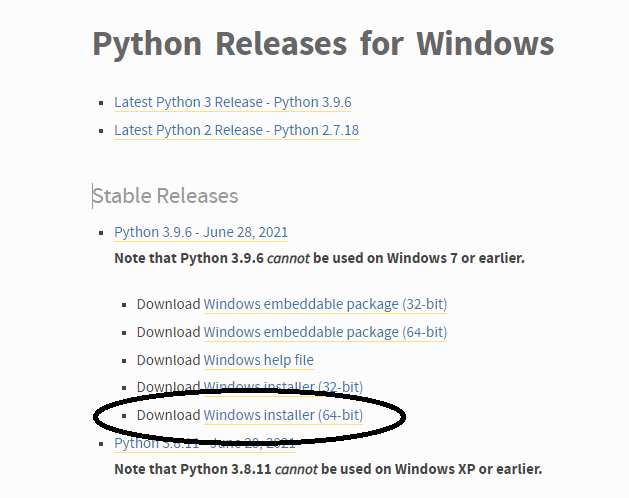
\includegraphics[width=10cm]{images/image11.png}

\begin{itemize}
	\item ・Download Windows x86 executable installer (32bit版)
	\item ・Download Windows x86-64 executable installer(64bit版)

\end{itemize}



いずれかを選択しダウンロードしますが、通常は32bit版であれば汎用性が高いです。


\includegraphics[width=10cm]{images/image8.png}

※画面は64bit版の3.6.2です。
\begin{enumerate}	
	\item 「Add Python 3.x to PATH」 をチェックしてください。
	\item Install now をクリックしてインストールをしてください。
\end{enumerate}

\subsection{エディター(vscode)準備}

次のURLを参照し「vscode」をダウンロードを行います。

\begin{description}
	\item $https://code.visualstudio.com/download$
\end{description}

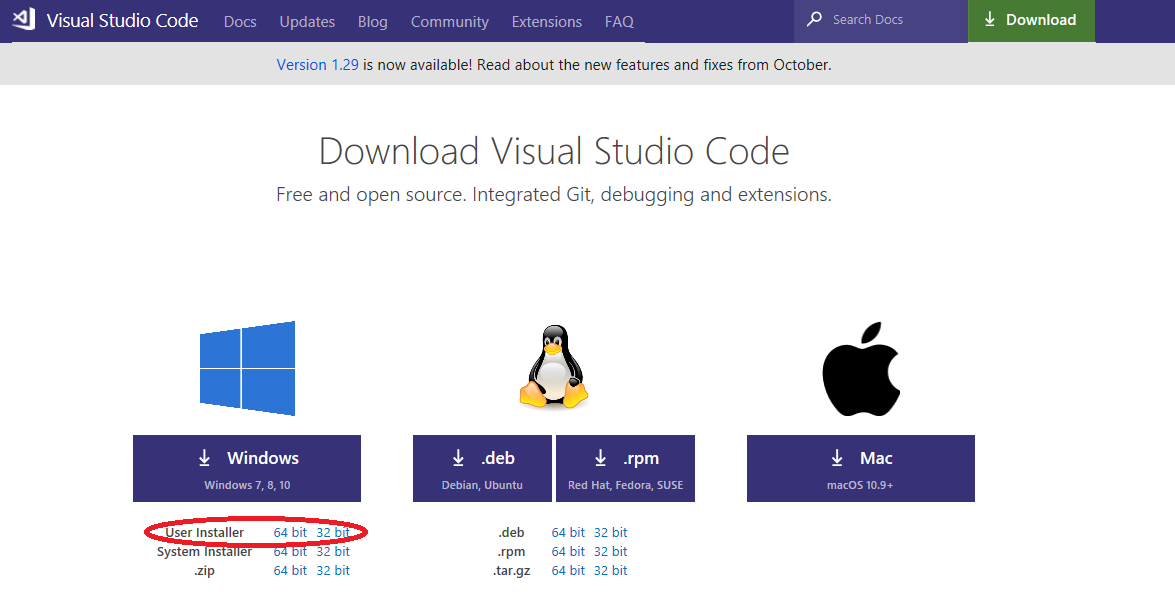
\includegraphics[width=10cm]{images/image9.png}

User Installerでそれぞれ32bit,64bitのいずれかを選択します。

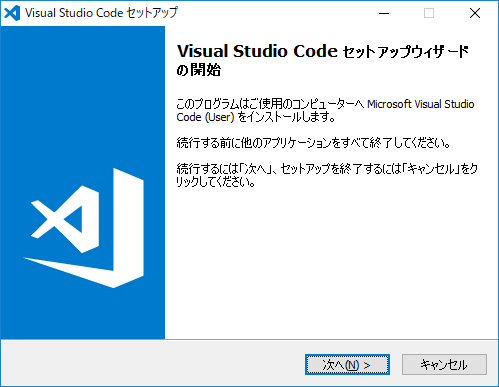
\includegraphics[width=10cm]{images/image12.png}


あとはインストールするだけです。

\subsubsection{vscodeの環境設定}

今回のプログラミングで利用するpythonの拡張機能をインストールします。

日本語表示のために日本語拡張機能のインストールを行います。



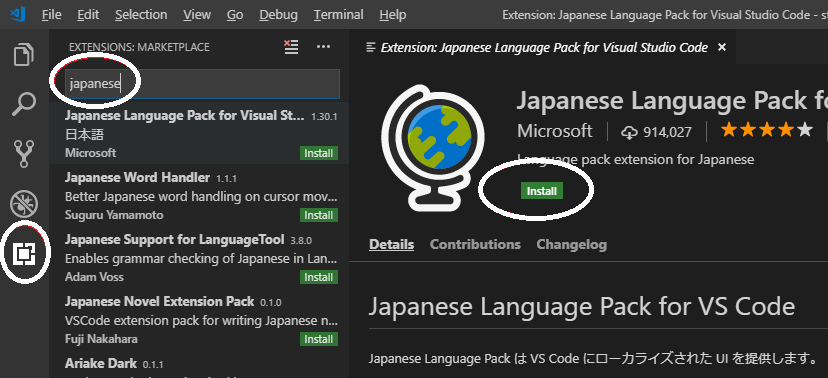
\includegraphics[width=10cm]{images/image2.png}

起動画面左下の拡張機能をクリックし、検索キーワードに「japanese」と入力し
「japanese Language Pack for Visual.....」を選択し「install」します。


ここでvscodeを再起動します。


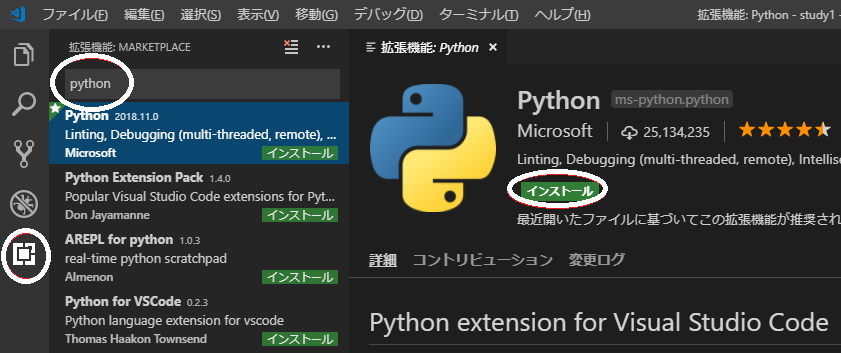
\includegraphics[width=10cm]{images/image6.png}

次に日本語拡張機能と同様に検索キーワードに「python」を入力することで今回プログラミングで利用するpythonの拡張機能をインストールします。

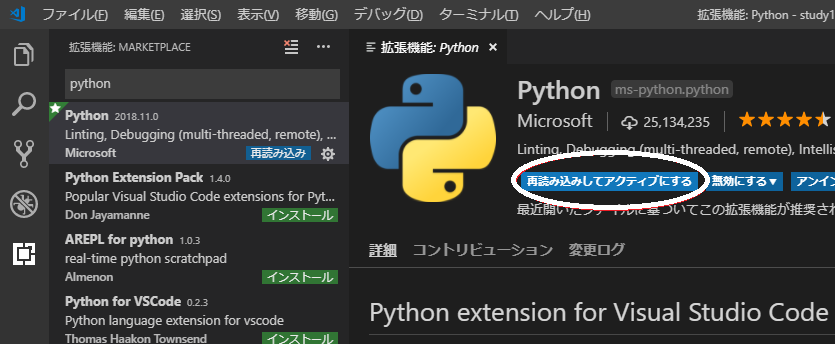
\includegraphics[width=10cm]{images/image10.png}

インストール後に
再読み込みしてアクティブにするを選択してpython拡張を有効にします。


これでインストールは完了です。




\chapter{プログラミング 最初の一歩}
\setcounter{section}{0}

\section{コンピューターへの命令の実行}
\subsection{命令や計算の実行方法}
 一つ一つ結果を確認して実行する方法と手順をたくさんまとめて実行する方法があります。

 コンピューターとは電気電子の作用によって動作する汎用計算機と訳されます。

\subsection{計算をさせてみよう。}

 まずは {\gt 対話実行}を行ってみましょう。

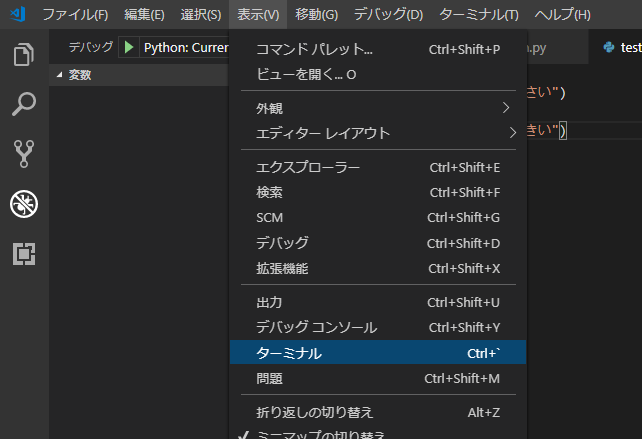
\includegraphics[width=10cm]{images/image1.png}

vscodeの「表示」メニューから「ターミナル」を選択します。

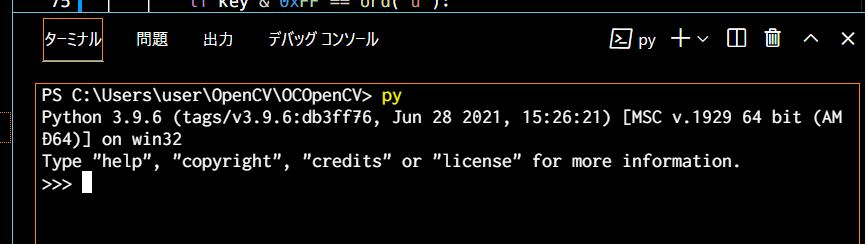
\includegraphics[width=10cm]{images/image7.png}

こちらの図のコマンドから「py」コマンドを起動しましょう。

 {\gt 対話実行pythonの起動}
\begin{listingcont}
c:\\~> py
Python 3.7.~省略~ on win32
Type "help", ~省略~
>>> 1 + 2 #>>>の後に計算式を入力します。
3
>>> 3 * 4
12
>>> 1 / 3
0.3333333333333333
>>> 1 +  1 / 4 
1.25
>>> 4 ** 2
16
>>> ( 1 + 2 + 3 ) / 2
3.0
\end{listingcont}


ここまでのように算式を入力していくと正しい結果を得られることを確認することができます。

※ 計算結果が割り切れない場合に無限に続く少数ではないことを確認しておきましょう。
 結果は有限桁で表現されています。

\subsection{変数とは?}

プログラムでは単純な計算以外に処理の結果を次に引き渡して連続したまとまった処理を多なうことが多いです。

その際に変数といわれる計算結果を一時的に保存しておくためのデータ領域が使われます。

 変数とは値を格納するもので数学の方程式で出てくるx,yなどによく似ています。

早速先程の続きで変数に値を代入する方法を見てみましょう。

 {\gt 変数の確認}
\begin{listingcont}
>>> x = 10
>>> x
10
>>> x / 4
2.5
>>> y = x - 5
>>> y
5
\end{listingcont}

最初の行の「x = 10」はxと10が等しいという意味ではなく左辺xに右辺の10という数値を入れておくという意味になります。(代入といいます。)

\subsection{変数の名前付けルール}
それではここで変数に利用できる文字にはどのようなものがあるか次の表で確認しましょう。
\begin{table}[h]
 \begin{center}
    \caption{変数に使える文字}
\begin{tabular}{|p{10cm}|} \hline
a ~ z のアルファベット(大文字も可) \\ \hline
0 〜 9 の数字 \\ \hline
\_ (アンダースコア) \\ \hline
\end{tabular}
\end{center}
\end{table}


\begin{description}

\item ※ 最初の文字を数字にすることはできません。
\item ※ 予約語/キーワード(ifやforなど・・・)と同じ名前は使えません。

\end{description}
 先程の「=」は代入という考え方なので次のように左辺10に右辺xを代入という考え方になってしまう式はエラーとなります。


 {\gt イコールの考え方等式}
\begin{listingcont}
>>> 10 = x
  File "<stdin>", line 1
SyntaxError: can't assign to literal
 ※ SyntaxError(エラー)になります。

>>> x = x - 1
>>> x
9
\end{listingcont}

等式として等しいという意味ではないので右辺の計算結果を左辺に代入という解釈を行います。したがって右辺には左辺に同じ変数を利用して
計算式を書くことができます。

 ※ =は右辺の式の値を左辺に代入という意味になります。

\subsection{式と計算}
 電卓では簡単にできないこんな計算もできます。
 {\gt 桁の多い計算}
\begin{listingcont}
>>> 2 ** 32
4294967296
>>> 2 ** 64
18446744073709551616
>>> 2 ** 128
(実行結果を確認してください)
  340澗2823溝6692穰0938じょ4634垓6337京4607兆4317億6821万1456
>>> 2 ** 256
(実行結果を確認してください)
  !?(無量大数を超えます)
\end{listingcont}


ここまでであればExcelでもできそうです。
\newline
{\gt Point}
 その他の計算、平方根(ルート)など一部の複雑な計算は別の仕組みを使います。したがってこのテキスト(授業)では触れません。



\section{まとまった手順の実行}
もっと手順について考えてみましょう。

それではまとまった手順を実行するスクリプト(簡易的な)プログラミングを行っていきましょう。\\

※本格的プログラミングは何千行・何万行・何十万行の命令を書いていきます。\\
10万行のプログラムを1ページ100行の印刷すると1000ページです。(小規模なプログラムでもこのくらいの量になります)

\subsection{一連の処理}
1~5までの合計(1 + 2 + 3 + 4 + 5)を計算するプログラムを実行しましょう。

 {\gt 同じような手順の繰り返し}
\begin{listing}{1}
>>> x = 1 
>>> x = x + 2
>>> x = x + 3
>>> x = x + 4
>>> x = x + 5
>>> x
15
\end{listing}

※ ヒント「↑」キーを押すと前の行が表示され編集をすることができます。

ここではプログラムで画面に出力する方法を学びます。
いままでも {\gt 対話実行}では結果の出力はできていましたが、明示的に出力する方法を学びます。


\subsection{画面に出力する方法}
結果を出力するprint文を使ってみます。
 {\gt 出力命令}
\begin{listingcont}
>>> print(x)
15
>>> x
15
\end{listingcont}

「print(x)」も「x」もxの値が出力されます。違いについては次のセクション「ファイルに保存」の中で説明します。


\subsection{ファイルへの保存}
これらのプログラムをひとまとまりの処理として書いてファイルに保存してみましょう。

\subsubsection{新規ファイルの作成}

ファイル名:python1-1.pyとして保存します。

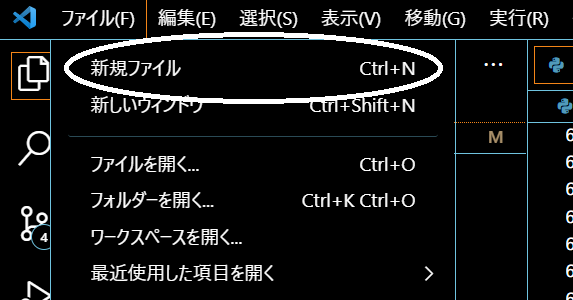
\includegraphics[width=10cm]{images/image5.png}


vscodeの「ファイル」メニュー「新規ファイル」を選択します。

エディターで次のプログラムを入力します。行番番号は自動で附番されます(プログラムの実行に影響はありません)ので、参考にしてください。

 {\gt 保存プログラム(python1-1.py)}
\begin{listing}{1}
x = 1
x = x + 2
x

\end{listing}

入力が完了しましたら保存の操作を行います。

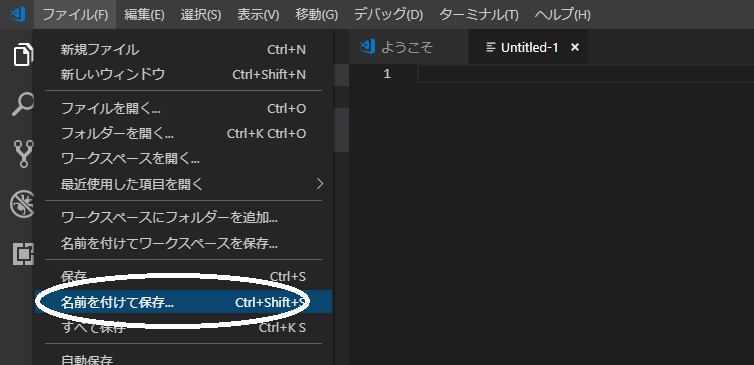
\includegraphics[width=10cm]{images/image4.png}

vscodeの「ファイル」メニュー「名前を付けて保存...」を選択します。

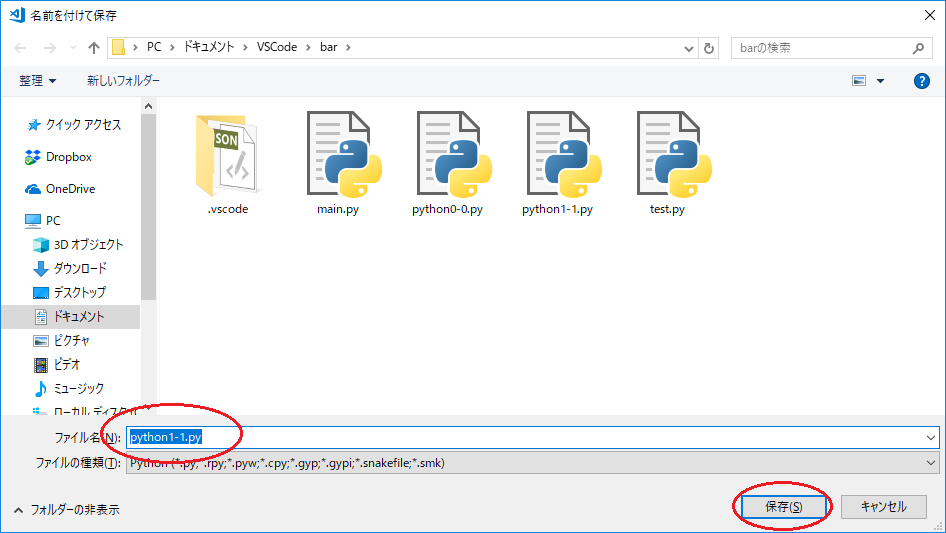
\includegraphics[width=10cm]{images/image13.png}

ファイル名「python1-1.py」と入力して保存を選択します。

保存が完了しましたら、{\gt 対話実行}で利用したターミナルに切り替えます。
\newline

{\gt Point}

{\gt 対話実行}で動作している場合はターミナルで「$>>> $」の後に、CTRL+Zを押すか「exit()」を実行することでコマンド実行状態に変更できます。

 {\gt 出力なしの実行}
\begin{listing}{1}
c:\\~> python python1-1.py
c:\\~>
\end{listing}

※ 計算はされていますが、表示されません。

それでは出力を行うためにもう一度ファイルを作成しprint文を追加してみましょう。

※ ファイル作成の手順は新規ファイルの作成を参照してください。

ファイル名:python1-2.py
 {\gt 保存プログラム(python1-2.py)}
\begin{listing}{1}
x = 1
x = x + 2
x = x + 3
print (x)
\end{listing}


実行方法
 {\gt 出力ありの実行}
\begin{listing}{1}
c:\\~> python python1-2.py
6
\end{listing}

※ 計算結果が表示されました。


まとまった手順をプログラムとして書いた場合、結果を出力する手続きを実行しなければ出力されません。プログラムで結果を出力する方法は「print関数」を利用することを覚えておきましょう。


※ {\gt 対話実行}で変数の値を出力するために変数名だけでよかった理由は式の評価した値が表示されたためです。

 評価についてはもう少し先に進めてから確認します。

\subsubsection{練習問題}
{\gt Plactice} \\
底辺xを3cm、高さyを4cmとする三角形の面積を求め出力するプログラムを作成しましょう。

ファイル名「plactice1.py」として保存しましょう。



\section{変数と式の評価}


もう一度{\gt 対話実行}で動作確認しています。
 {\gt 式}
\begin{listing}{1}
c:\\~> py
>>> x = 1
>>> x
1
\end{listing}

※ ここまでは復習です。
\subsection{式の評価}
ここで式(条件式)の評価について学びます。(まずは不等号から)
 {\gt 式の評価}
\begin{listingcont}
>>> x < 10
True
>>> x > 10
False
\end{listingcont}

※ 条件式が成立していると「True」が不成立であれば「False」になっていることがわかります。

\newpage 
条件式で利用される主なもの式の書き方
\begin{table}[h]
 \begin{center}
    \caption{条件式(比較演算子)}
\begin{tabular}{|c|p{4cm}|} 
\hline
記号 & 意味 \\ \hline \hline
 $ == $ & “等しい” \\ \hline
 $ < $ & “小なり” \\ \hline
 $ > $ & “大なり” \\ \hline
 $ <= $ & “小なりイコール” \\ \hline
 $ >= $ & “大なりイコール” \\ \hline
 $ != $ & “等しくない” \\ \hline
\end{tabular}
\end{center}
\end{table}


それでは条件式を使った式の評価を見ていきましょう。
 {\gt 式の評価(条件式1)}
\begin{listingcont}
>>> x <= 1
True
>>> x >= 2
False
>>> x == 1
True
>>> x == 2
False
>>>  x != 1
False
\end{listingcont}


当たり前ですが、こんな式の評価もできます
 {\gt 式の評価(条件式2)}
\begin{listingcont}
>>> 60 < 70
True
>>> 60 > 70
False
\end{listingcont}

ほかの言語では書けないかもしれませんが次のような式の条件式も可能です。
 {\gt {式の評価(条件式3)}}
\begin{listing}{1}
>>> x = 5
>>> 1 < x < 10
True
>>> 1 < x < 5
False
\end{listing}

※ ほかの言語では「1 $<$ x and 1 $<$ 10」など「かつ」条件で記入することが多いです。

文字や文字列も比較できます。
 {\gt {式の評価(条件式4)}}
\begin{listing}{1}
>>> a = "z"
>>> b = "z"
>>> a == b
True
>>> c = "y"
>>> a == c
False
>>> a > c # "z" > "y" を辞書順で評価します。
True
>>> a < c
False
>>> a = "abc"
>>> b = "abc"
>>> c = "azc"
>>> a == b
True
>>> a == c
False
>>> a > c # "abc"と"azc"の辞書順の評価
False
>>> a < c
True
\end{listing}

{\gt Point}

 {\gt 対話実行}で表示されている「$>>>$」の後に入力する命令や式は実行され「評価」されます。


 {\gt 変数の評価}
\begin{listing}{1}
>>> x = 1
※ xに1を代入するという命令が実行された。
>>> x
1
※ xを評価した結果が表示された。
>>> print ( x )
1
※ xを表示する命令が実行された。
\end{listing}


このように {\gt 対話実行}では条件式や計算式の評価結果を表示しますので、print命令による出力と違いがわかりません。
プログラムをファイルに保存して実行する場合は条件式や計算式の評価結果は出力されませんので、print命令によって明示的に出力する必要があります。

\subsection{if文(場合分けの処理)}

評価について理解できてきたと思います。評価は場合分けで利用するために行われます。

条件が成立した(式の評価が真)のときに行う手続き、不成立(式の評価が偽)のときに行う手続きをまとめて記述します。


 {\gt if文の書き方1}
\begin{listing}{1}
if 条件式:
    真の手続き1
    真の手続き2
    ・
    ・
else:
    偽の手続き1
    偽の手続き2
    ・
    ・
\end{listing}

{\gt Point}
「python」ではまとまった手順を「プロック」といい、共通のインデント(左端からの字下げ)で表します。
ブロックを書くときは「行末」に{\underline{\tt 「:」}}を書く必要があります。

※ 「真の手続き」「偽の手続き」は「タブ」や「スペース」で字下げ(インデント)することで複数の手続きをひとまとまりのブロックにすることができます。


それではifによる場合分けを確認しましょう。

{\gt 凡例if-1}

変数xに学生Aさんの数学の得点を入力します(今回は60点とします)。このテストでは50点以上を合格としますので、Aさんの数学の得点が合格なのか不合格なのか判定して出力するプログラムを作りましょう。

※ ここでは {\gt 対話実行}で場合分けの処理を実行してみます。

{\gt プログラムif-ex.py}
\begin{listing}{1}
>>> x = 60
>>> if x >= 50:
...      print ( " goukaku " ) # 左側のインデント空白は
                                 「Tab」キー(1回)で入力します。
... else:
...      print ( " fugoukaku " )
... #インデントなしで「Enter」キーを押すと式を評価して結果を
     表示します。
goukaku
>>>
\end{listing}



\begin{description}
 \item print命令で文字を出力するときは「"」(ダブルクォーテーション)や「'」(シングルクォーテーション)で文字を囲む必要があります。(変数と区別するためです。)
\end{description}


if文の意味が理解出来たらまとまった手順としてプログラムを作ってみましょう。

\subsubsection{練習問題}
{\gt Plactice} \\
新規ファイルを作成して「凡例if-1」を保存して実行してみましょう

ファイル名「plactice2.py」として保存しましょう。


他にもif文の書き方はいくつかありますので、確認してみましょう。

if文では真の手続きのみ必要で偽の手続きを記載する必要の無い場合があります。
その時のif文は書き方2を確認してください。
 {\gt if文の書き方2(偽の手続きがない場合)}
\begin{listing}{1}
if 条件式:
    真の手続き1
    真の手続き2
    ・
\end{listing}

このときのブロックは複数行書くことができます。if文が終了後はインデント無しで次の行から命令を書いていきます。

また、if文には1つの条件が偽の場合2つ目、3つ目の条件が真の場合に実行あるいはすべての条件に当てはまらない時の実行を書くことができます。

 {\gt if文の書き方3(条件1にあっているとき、条件2にあっているとき・・・・・)}
\begin{listing}{1}
if 条件式1:
    条件式1が真の手続き
    ・
elif 条件式2:
    条件式1が偽で条件式2が真の手続き
    ・
elif 条件式3:
    条件式1~2が偽で条件式3が真の手続き
    ・
else:
    条件1~3が偽の時の手続き
    ・
\end{listing}

\newpage
それではifを使って判定するプログラムを作ってみましょう。
{\gt 凡例if-2}
変数xに学生Aさんの数学の得点を入力します(今回は60点とします)。このテストでは80点以上を「A」とし、60点以上を「B」とし、40点以上を「C」、40点未満を「D」と評価します。Aさんの数学の得点の評価を判定して出力するプログラムを作りましょう。
ファイル名:python2-2.pyとして保存し実行しましょう。
{\gt プログラムputhon2-2.py}
\begin{listing}{1}
x = 60
if x >= 80:
    print ( “A” )
elif x >= 60:
    print ( “B” )
elif x >= 40:
    print ( “C” )
else:
    print ( “D” )
\end{listing}

保存しif文の動作を確認してみましょう。

※ xに代入されている得点をA,B,C,Dそれぞれに該当する値にして実行してみましょう。


if分だけで完結するのではなくその後のプログラムに値を引き渡すプログラムを作成してみましょう。
{\gt 凡例if-3}
凡例「if-2」を評価メッセージA判定なら「"excellent"」、B判定なら「"good"」、C判定なら「"passing"」、D判定なら「"failing"」と変数mesに代入し出力する
プログラムを作成しましょう。

ファイル名:python2-3.pyとして保存し実行しましょう。
{\gt プログラムputhon2-3.py}
\begin{listing}{1}
x = 60
if x >= 80:
    mes = "excellent"
elif x >= 60:
    mes = "good"
elif x >= 40:
    mes = "passing"
else:
    mes = "failing"

print mes
\end{listing}


※ xに代入されている得点をA,B,C,Dの判定にそれぞれに該当する値にして実行してみましょう。

\subsubsection{練習問題}
{\gt Plactice} \\
変数xと変数yにそれぞれ整数を代入してxの値が大きければ"x is large."と表示し、
yの値が大きければ"y is large."と表示、等しければ"x and y are equal."と
表示するプログラムを作りましょう。

ここでxとyはプログラム中でそれぞれ値を入れてif文が正しく動作することを確認しましょう。
ファイル名「plactice3.py」として保存しましょう。

\subsection{if文(複合条件)}
複数の条件が関係する条件式も利用することができます。

例えばテストの点数が0点以上と100点以下であることを判定するための条件(複合条件と言います)の記載方法もあります。

 {\gt 条件式の書き方(複合条件)}
\begin{verbatim}
1.条件式1と条件式2がともに真の時「かつ」
  条件式1 and 条件式2
2.条件式1と条件式2のどちらかが真の時「または」
  条件式1 or 条件式2
3.条件式の判定が偽の時「否定」(わかりにくいですが)
    not 条件式
\end{verbatim}



 {\gt 対話実行}で「and or not」条件の評価を確認しましょう。

 {\gt and or notの式の評価}
\begin{listing}{1}
>>> x = 999
>>> x > 100
True
>>> not x > 100
False
>>> x >= 0 and x <= 100
False
>>> x < 0 or x > 100
True

\end{listing}

※式の評価について確認ができたと思います。


それではif文を使った練習問題をやってみましょう。

\subsubsection{練習問題}
{\gt Plactice} \\
「凡例if-2」を101点以上、0点未満の場合「error」と表示されるプログラムに変更してください。

ファイル名「plactice4.py」として保存しましょう。


\section{キーボードからの入力}
プログラムを実行時に変数に値をキーボードから入力した値に実行後設定してみましょう。このような値の代入を動的な値の代入といいます。

 {\gt 対話実行}してキーボードからの入力をしてみましょう。
 {\gt キーボードからの入力}
\begin{listing}{1}
>>> input()
abc # キーボードから入力
‘abc’
>>>
>>> input( “type = ” )
type = xyz
‘xyz’
>>>
\end{listing}


※ 入力した文字が評価されて表示されました。

入力した文字を変数sにいれてみましょう。
 {\gt キーボードから変数への代入}
\begin{listingcont}
>>> s = input( “type = “ )
type = xyz
>>> s
‘xyz’
>>>
\end{listingcont}

※変数sに文字が入力されていることを確認できました。

\subsection{文字列の取り扱いについて}

文字列は「"」(ダブルクォーテーション)や「'」(シングルクォーテーション)で囲まれ数値とは異なる扱いになります。
ここでは文字列と数値の違いを確認してみましょう。
 {\gt 文字列の取り扱い}
\begin{listingcont}
>>> s * 2
‘xyzxyz’
※ 同じ文字列が2倍になりました
>>> s + 10
Traceback (most recent call last):
  File "<stdin>", line 1, in <module>
TypeError: can only concatenate str (not "int") to str
※ 文字列と数値では計算できませんのでエラーになります。
>>> s + “10”
xyz10
※ 文字列と文字列はプラスで連結されることがわかります。
\end{listingcont}


それでは入力した数値を使って計算する方法を学んでみましょう。

キーボードから入力された数字は数値ではなく文字として認識されていることを確認しましょう。

 {\gt 文字列の取り扱い(数字1)}
\begin{listingcont}
>>> s = input ( “number = “ )
10
>>> s
‘10’
>>> s * 2
‘1010’
※ このままだと変数sは文字列の’10’が入っています。
\end{listingcont}

\subsubsection{文字列から数値への変換}
文字として入力された数字(文字列)を数値に変換するためにはint命令を利用します。
 {\gt 文字列の取り扱い(数値への変換)}
\begin{listingcont}
>>> int(s)
10
※ シングルクォーテーションがなくなりました。
>>> n = int(s)
>>> n * 2
20
※ 数値として評価されています。
\end{listingcont}

{\gt Point}
数値として判定できない文字の扱いはエラー処理(例外処理)として別に考える必要があります。

\subsubsection{数値から文字列への変換}
数値を文字列にするにはstr命令を利用します。
 {\gt 数値から文字列のへの変換}
\begin{listingcont}
>>> str( n * 2 )
‘20’
>>> str( n * 2 ) + “ is twenty”
‘20 is twenty’
\end{listingcont}

文字列にすると「+」演算子で連結(文字列を結合すること)もできます。

{\gt 凡例input-1}
学生Aさんの数学の得点をxに、英語の得点をyに入力し数値化して平均点を出力しましょう。(数値化後の変数をそれぞれmとeを使います)

ファイル名:python4-1.pyとして保存し実行しましょう。

※ 入力が数値として判定できない場合の処理は行いません。
{\gt プログラムpython4-1.py}
\begin{listing}{1}
x = input ( “math = “ )
m = int ( x ) 
y = input ( “english = “ )
e = int ( y )
print ( “The average score is “ + str ((m + e) / 2) )
\end{listing}
実行結果
\begin{listing}{1}
math = 50
english = 80
The average is 65.0
\end{listing}



※ 数値以外のものを入力するとエラーになりますのでご注意ください。


\subsubsection{練習問題}
{\gt Plactice} \\

「凡例input-1」を社会の得点をzに入力「”{\tt social = }“」し、変数sに数値化して学生Aさんの1科目当たりの平均点を出力しましょう。

python4-1.pyをファイル名「plactice5.py」として別名で保存しましょう。
\newline 
{\gt Point}

変数名について

変数名は変数が少ない時は一文字のアルファベット「a ~ z」でも問題ないですが、長い手順になってくると意味を持たない文字列では分かりにくくなります。
そこで少しずつ分かりやすい変数名をつけていくことを意識していきましょう。

\newpage
\section{繰り返し処理}
ここからは繰り返し処理について学びます。
コンピューターはどんなに同じことを繰り返しても文句ひとつ言いません。これがコンピューターを利用する大きな理由になっています。

\subsection{for文による繰り返し}
プログラミングでは繰り返し処理をする方法が用意されています。



{\gt 凡例for-1}

for文を使って3回”wan” ”nyan”と表示します。

ファイル名をpython5-1.pyとして保存しましょう。
{\gt プログラムpython5-1.py}
\begin{listing}{1}
for x in range(3):
    print( “wan” )
    print( “nyan” )
\end{listing}
実行結果
\begin{listing}{1}
wan
nyan
wan
nyan
wan
nyan
\end{listing}



※ range()の括弧中に書かれている回数繰り返していることがわかります。


for文はブロック内に書かれている処理をrangeの中に書かれている回数だけ繰り返しすることが理解できたと思います。
\subsubsection{練習問題}
{\gt Plactice} \\
同じく1000回”wan” "nyan"と表示させましょう。

python5-1.pyをファイル名「plactice6.py」として別名で保存しましょう。






\subsubsection{rangeによる値のリスト}
for文ではinの後ろに書かれているrange()の括弧中に書かれている数値をinの前に書かれている変数に
値を代入しながら値がなくなるまで繰り返しする命令です。

では具体的に代入される値を確認してみましょう。
{\gt 凡例for-2}

for文の次に書いているのは変数xです。


変数xの値を表示してみましょう。

ファイル名:python5-2.py

{\gt プログラムpython5-2.py}
\begin{listing}{1}
for x in range(3):
    print( x )
\end{listing}

実行結果
\begin{listing}{1}
0
1
2
\end{listing}


変数xにはrange命令で指定された範囲の値がひとつずつ入っていることが分かりました。range命令ではどのような値が
展開されるかは次の通りとなります。
\begin{description}
\item range(3)・・・ 0,1,2
\item range(5)・・・ 0,1,2,3,4
\end{description}
※ 「0」から括弧の中にある数値-1までの範囲の値が作られます。

{\gt 凡例for-3}
凡例for-3

それぞれ次のrange命令で指定するとどんな値が入っているか確認してみましょう。
\begin{description}
\item {\tt range(1, 5)}
\item {\tt range(1, 10)}
\item {\tt range(1, 10, 2)}
\item {\tt range(2, 10, 3)}
\end{description}
 {\gt 対話実行}してみましょう。

{\gt プログラム対話実行}
\begin{listing}{1}
>>> for x in range(1, 5):
...     print( x )
...
1
2
3
4
	・
	(中略)
	・
>>> for x in range(2, 10, 3):
...     print( x )
...
2
5
8
\end{listing}


このようにrange()で作られる値は最初の値が初期値、2つ目の値が上限値(未満となるよう)、3つ目の値を加算していくため、次のようになることがわかります。
\begin{description}
\item {\tt range(1, 5)} $\rightarrow$ {\tt 1, 2, 3, 4}
\item {\tt range(1, 10)}	$\rightarrow$	{\tt 1, 2, 3, 4, 5, 6, 7, 8, 9}
\item {\tt range(1, 10, 2)}	$\rightarrow$ {\tt 1, 3, 5, 7, 9}
\item {\tt range(2, 10, 3)}	$\rightarrow$ {\tt 2, 5, 8}
\end{description}
括弧の中で指定している最初の値から次の値-1まで最後の値が加算された値が取得されます。

\newpage
{\gt 凡例for-4}

1から10までの数値を足した合計を求めるプログラムを作りましょう。

ファイル名をpython5-3.pyとして保存してください。
{\gt プログラムpython5-3.py}
\begin{listing}{1}
sum = 0
for x in range(10):
    sum = sum + x
print ( sum ) 
\end{listing}


\subsubsection{練習問題}
{\gt Plactice} \\
1.「凡例for-4」を改良して1から1000までの数値を足した合計を求めるプログラムを作りましょう。

2.「凡例for-4」に追加して「アキレスと亀」(ゼノンのパラドックス)をやってみましょう。(詳しくはネットで検索しましょう)

※ 1/2 + 1/4 + 1/8 + 1/16 無限に計算すると値が収束することを確かめます。

 人間が計算するとすぐ嫌になりますが、コンピューターは音を上げません。

 ただしrangeで計算する数値の範囲が、2 ** 128あたりでどのくらいになるのか想像し

 てから実行してみてください。

※ (1 / 2 ** 53 )あたりまでで精度が足りなくなるみたいです。

python5-3.pyをファイル名「plactice7.py」として別名で保存しましょう。




\subsection{繰り返し処理の利用}
 繰り返しの中にキーボードからの入力を処理する機能をいれて、プログラムを短くしてみましょう。

先ほどの「凡例input-1」を10科目の平均表示に変更することを考えてみます。

※ 悪い例「人がやる繰り返し」です。変数名が増えますので、ちょっと手抜きします。
\newpage
 {\gt 人がやる繰り返し}
\begin{listing}{1}
x = input ( “subject1 = “ )
y = int ( x ) 
x = input ( “subject2 = “ )
y = y + int ( x ) 
x = input ( “subject3 = “ )
y = y + int ( x ) 
x = input ( “subject4 = “ )
y = y + int ( x ) 
※ そろそろ飽きてきます。
    ・
    ・
    ・
x = input ( “subject10 = “ )
y = y + int ( x ) 
print ( y / 10 )
※ できますが、電卓入力のほうが楽です。
\end{listing}


この問題を解決するために、効率よく繰り返しコンピューターに処理を行わせる方法を学びましょう。

よく見ると2科目目以降はそっくりです。

\begin{verbatim}
x = input ( “subject2 = “ )
y = y + int ( x ) 
\end{verbatim}

1科目目も0に入力した値を加算すると書き換えてみましょう。(初期値0という意味です。)
\begin{verbatim}
x = input ( “subject1 = “ )
y = 0 + int ( x ) 

つまり最初だけ変数yに0を入れます。
y = 0
ここから10回繰り返し
x = input ( “subjectN = “ )
y = y + int ( x )

繰り返しが終わったら平均値を出力します。
print ( y / 10 )
\end{verbatim}

{\gt 凡例for-5}
繰り返しを用いてシンプルに記述します。

ファイル名:python5-4.py
{\gt コードpython5-4.py}
\begin{listing}{1}
y = 0
for n in range(10):
    x = input ( “subjectN = “ )
    y = y + int( x )
print( y / 10 )
\end{listing}

※ こんなに短くできました。



プログラムを書くときは短く効率的に書くことを意識してくことが大切なことがわかります。

繰り返しはコンピュータにさせるべきで人間が繰り返し同じことを書かない方が良いといわれています。

\subsubsection{練習問題}
{\gt Plactice} \\
「凡例for-5」のプログラムの科目毎の点数入力の際「subject1~5 =」のように何番目の科目を入力しているのか分かりやすく表示してください。

python5-4.pyをファイル名「plactice8.py」として別名で保存しましょう。


\subsection{繰り返し処理のその他の制御}

繰り返しには他にもwhile文があります。

while文の書き方は次の通りですが、条件式(式の評価)が真の間繰り返すことになります。
\begin{verbatim}
while 条件式:
    手続き1
    手続き2
    ・
\end{verbatim}
基本的にはfor文と同様にwhile文以降のブロックを条件が真の間繰り返しますので、ブロック内で条件が偽になるような処理を記述する必要があります。
{\gt 凡例loop-1}
whileを使って1~5までの合計を求め出力するプログラムを作ります。

ファイル名:python5-5.py
{\gt コードwhileを利用したやり方}
\begin{listing}{1}
i = 1
total = 0
while i <= 5:
    total = total + i
    i = i + 1

print(total)
\end{listing}


繰り返し処理の途中で繰り返しを終了する制御文にbreakがあります。

break文を利用するとfor文やwhile文といった繰り返しを途中で終了することができます。

\begin{verbatim}
while 条件式:
    手続き1
    手続き2
        break #これで繰り返し文を抜けることができます。
\end{verbatim}

break制御を使うことで繰り返し処理を終了できますので、while文の条件式にTrueを設定
しても制御可能になります。
{\gt 凡例loop-2}
whileを使って1~5までの合計を求め出力するプログラムを作ります。
ここでwhile文は式の評価結果を常に真とするようにしています。

ファイル名:python5-6.py
{\gt コードwhileを利用したやり方}
\begin{listing}{1}
i = 1
total = 0
while True:
    total = total + i
    i = i + 1
    if i == 6:
        break

print(total)
\end{listing}



pythonの繰り返し処理には繰り返しが終了したタイミングで修了時の処理をするために
else:ブロックを利用することができます。

\begin{verbatim}
while 条件式:
    手続き1
    手続き2
else:
    条件式が偽になった時の手続き
\end{verbatim}
ただし、この処理は条件式が偽になる必要があるため、break文による制御で繰り返し処理を
終了した場合は、else:ブロックは通過しません。

また、他にはcontinue制御文もありますが、ここでは説明しませんので、興味があれば検索してください。

\section{配列について(繰り返し処理の活用)}

\subsection{配列とは?}

効率的に処理するために繰り返し処理と組み合わせてよく使われるのが配列です。配列の考え方は一覧(並び)に近いので一覧を表示することをイメージしてみます。

得点入力の科目名を一覧表示するプログラムは次の通りです。

何度も同じ科目名を入力したり出力するのであれば変数に入れておきますが、繰り返し同じことを書くのは非効率的です。
\newpage
 {\gt 変数の利用(繰り返し記述)}
\begin{listing}{1}
m = “Mathematics”
print ( m )
e = “English”
print ( e )
so = “Social”
print ( so )
j = “Japanese”
print ( j )
sc = “Scientific”
print ( sc )
\end{listing}


そこで繰り返し利用できるように、同じ変数に値の一覧として格納していきます。
 {\gt 配列の利用}
\begin{verbatim}
subjects = [“Mathematics”,”English”,”Social”,”Japanese”,”Scientific”]
\end{verbatim}
この変数{\tt subjects}に格納されている値のイメージは次の通りとなります。
 \begin{center}
\begin{tabular}{|c|p{5cm}|} \hline
      & 変数subjects(配列)       \\ \hline \hline
0番目  & “Mathematics”  \\ \hline
1番目  & “English”      \\ \hline
2番目  & “Social”       \\ \hline
3番目  & “Japanese”     \\ \hline
4番目  & “Scientific”   \\ \hline
\end{tabular}
\end{center}

ここで変数{\tt subjects}に格納されている値を参照するためには{\tt subjects[0]}と{\tt []}角括弧の中に何番目を
表す数値や数値の入った変数を利用することができます。

つまり変数subjectsの中の"English"を参照するためには1番目を参照すればよいので{\tt subjects[1]}と記述します。
\newline 
{\gt Point}
配列を番号で参照するときの番号を「添字」もしくは「インデックス」と呼びますので覚えておきましょう。

\newpage
for文と配列を使って効率よく出力処理してみましょう。

{\gt 凡例list-1}

配列listを使って5科目を一覧表示してください。

ファイル名:python6-1.py
{\gt プログラムpython6-1.py}
\begin{listing}{1}
subjects = [“Mathematics”,”English”,”Social”,”Japanese”,”Scientific”]
for s in subjects:
    print ( s )
\end{listing}
実行結果
\begin{listing}{1}
Mathematics
English
Social
Japanese
Scientific
\end{listing}

for文ではinの後ろにある配列(list)の内容を最後まで繰り返し処理することができます。

for文では配列の最初の値を変数に代入してブロック内の処理します。次に配列の次の値を変数に代入してブロック内の処理をします。
配列の中身をすべて変数に代入し、次の処理すべき配列がなくなったときに処理を終了します。

つまり変数{\tt s}の中身は“Mathematics”$\rightarrow$”English”$\rightarrow$”Social”$\rightarrow$”Japanese”$\rightarrow$”Scientific”と
変化しながらブロック内の処理「{\tt print ( s ) }」を実行することになります。
\newpage
for文と配列を使ってデータ入力と出力を効率よく処理する流れを見てみましょう。
{\gt 凡例list-2}

配列(リスト)を使って5科目を一覧表示し、科目の点数を配列scoresに入力して、一覧表示してください。

ファイルpython6-1.pyをpython6-2.pyにコピーにして保存してください。
{\gt プログラムpython6-2.py}
\begin{listing}{1}
subjects = \
        [“Mathematics”,”English”,”Social”,”Japanese”,”Scientific”]
scores = [] 
for s in subjects:
    x = input( s + “ = “ )
    y = int ( x )
    scores.append( y )

l = len(subjects)
#配列の長さはlen関数を利用することで求められます(ここでは5となります)
for n in range(5):
    print ( subjects[n] + “:” , scores[n])
# print命令は「,」(カンマ)でつなぐと改行なしで値を出力できます。
\end{listing}


※ プログラム中のコメント(プログラムの説明文)は「\#」以降となり実行に影響を与えません。


配列リストは自由に要素を追加削除できます。

{\tt scores = []}

この文では変数scoresが配列であることを宣言しています。

{\tt scores.append( y )}

この文は配列に値を追加しています。(任意の値を追加していくことができます)
\newline {\gt Point}
また、何度か追加したリストの長さは{\tt len}関数の括弧の中に記述することで長さが取得できます。

この配列(リスト)はイメージとして次のようになります。
\newpage
\begin{table}[h]
 \begin{center}
    \caption{配列のイメージ}
\begin{tabular}{|c|c|c|} \hline
      & subjects      & scores \\ \hline \hline
0番目  & “Mathematics” &   10	\\ \hline
1番目  & “English”     &   20 \\ \hline
2番目  & “Social”      &   30 \\ \hline
3番目  & “Japanese”    &   40 \\ \hline
4番目  & “Scientific”  &   50 \\ \hline
\end{tabular}
\end{center}
\end{table}


値を参照するためには配列名[番号]で利用することができますので、科目名と点数の一覧は次の命令で出力させることができます。

 {\gt 繰り返し出力}
\begin{listing}{1}
for n in range(5):
    print ( subjects[n] + “:” , scores[n])
\end{listing}
この時の変数nの値は0,1,2,3,4とれぞれ繰り返しの中で変化していきますので、
出力結果は次の通りとなります。
\begin{listing}{1}
Mathematics: 10
English: 20
Social: 30
Japanese: 40
Scientific: 50
\end{listing}

for文と配列、if文を組みああせて行う処理を学んでみましょう。
{\gt 凡例list-3}

「凡例list-2」の繰り返しの中で得点が60点以上は”合格”、60点未満は”不合格”と表示するように変更してみましょう。

ファイルpython6-2.pyをpython6-3.pyにコピーにして保存してください。
{\gt プログラムpython6-3.py}
\begin{listing}{1}
subjects = \
        [“Mathematics”,”English”,”Social”,”Japanese”,”Scientific”]
scores = [] 
for s in subjects:
    x = input( s + “ = “ )
    y = int ( x )
    scores.append( y )

for n in range(0,5):
    if scores[n] >= 60:
        mes = “合格”
    else:
        mes = “不合格”
    print ( subjects[n] + “:” , scores[n], mes)
\end{listing}



\subsubsection{練習問題}
{\gt Plactice} \\
ここまでの学習内容を復習して5科目の点数を入力し、0点未満や100点を超える点数は「error」と表示し入力された場合は得点に-1を設定するようにしましょう。

5科目の点数を入力完了したら、このテストでは80点以上を「excelent」とし、60点以上を「good」とし、40点以上を「passing」、40点未満を「failing」と評価します。5科目の得点の評価を判定して出力するプログラムを作りましょう。

エラーと表示された科目については「error」と出力します。

python5-1.pyをファイル名「plactice9.py」として別名で保存しましょう。

{\gt コード実行例}
\begin{verbatim}
c:\\~> py plactice9.py
Mathematics = 50
English = 60
Social = 80
Japanese = 39
Scientific = 101
error

Mathematics: 50 passing
English: 60 good
Social: 80 excelent
Japanese: 39 failing
Scientific: -1 error
\end{verbatim}



\subsection{2次元配列}


3×2の配列(リスト)を作ってみましょう。
学生3人の数学と英語の点数を管理する方法を考えます。
\begin{description}
\item Aさんの数学(60)と英語(80)
\item Bさんの数学(70)と英語(90)
\item Cさんの数学(80)と英語(100)
\end{description}

\begin{verbatim}
math = [60, 70, 80]
english = [80, 90 ,100]
a = [60, 80]
b = [70, 90]
c = [80, 100]
\end{verbatim}

どちらの考え方も間違っていませんが、科目が増えたり人数が増えたときに効率よく扱うことができません。
\newpage
\subsubsection{2次元配列の宣言}

一人分のデータをリストとしてさらにリストの中に入れることができます。

\begin{verbatim}
students_scores = [[60, 80], [70, 90], [80, 100]]
\end{verbatim}
\begin{table}[h]
 \begin{center}
    \caption{二次元配列}
\begin{tabular}{r|c|r|r|} 
 & & 0列目 &1列目\\ \hline 
 & & 数学 &英語\\ \hline 
0行目 & Aさん &  60& 80\\ \hline
1行目 & Bさん &  70& 90\\ \hline
2行目 & Cさん &  80& 100\\ \hline
\end{tabular}
\end{center}
\end{table}

Aさんの数学の点数(60点)は配列{\tt students\_scores[0][0]}で参照できます。
同様にBさんの数学の点数(70点)を参照するには{\tt students\_scores[1][0]}、Cさんの英語の点数(100点)を参照するには
{\tt students\_scores[2][1]}と表現します。

\subsubsection{データの追加(行)}

Dさんのデータ(数学 50点, 英語 70点)が増えたときは{\tt students\_scores}にDさんの配列{\tt [50, 70]}を次のように追加します。


\begin{verbatim}
students_scores.append([50, 70])

配列の中身:[[60, 80], [70, 90], [80, 100], [50, 70]]
\end{verbatim}

\subsubsection{データの追加(列)}

Aさんの3科目目(社会科 70点)を追加するときはAさんのデータ{\tt students\_scores[0]}に{\tt append}します。

\begin{verbatim}
students_scores[0].append(70)

配列の中身:[[60, 80, 70], [70, 90], [80, 100], [50, 70]]
\end{verbatim}

\begin{table}[h]
 \begin{center}
    \caption{二次元配列操作後}
\begin{tabular}{r|c|r|r|r|} 
 & & 0列目 &1列目& 2列目\\ \hline 
 & &数学&英語&社会\\ \hline \hline
0行目 &Aさん &  60& 80 & 70 \\ \hline
1行目 &Bさん &  70& 90 & \\ \hline
2行目 &Cさん &  80& 100 & \\ \hline
3行目 &Dさん &  50& 70 & \\ \hline
\end{tabular}
\end{center}
\end{table}

\newpage
\subsubsection{2次元配列を利用した集計}
{\gt 凡例list-4}
2次元配列の例で利用した{\tt students\_scores = [[60, 80], [70, 90], [80, 100]]}(数学と英語の点数)
を使って科目の合計点を求めるプログラムを作成しましょう。

ファイル名をpython6-4.pyとして保存してください。
{\gt プログラムpython6-4.py}
\begin{listing}{1}
students_scores = [[60, 80], [70, 90], [80, 100]]
m = 0 #数学の合計点
e = 0 #英語の合計点

for v in students_scores:
    m = m + v[0]
    e = e + v[1]

print ("数学の合計点数", m)
print ("英語の合計点数", e)
\end{listing}
実行結果
\begin{listing}{1}
数学の合計点数 210
英語の合計点数 270
\end{listing}

この判例のfor文ではinの後ろにつく配列{\tt students\_scores}は3人分の数学と英語の点数が入っているので
一人分のデータをvに代入することになります。
この一人分のデータは数学と英語の得点の配列となりますので、{\tt v[0]}(数学の点数){\tt v[1]}(英語の点数)として参照することができます。

また二次元配列を参照しながら処理を行うには添字を使う方法もあります。
{\gt 凡例list-5}
添え字を使って前の凡例と同「list-4」じ機能を作ってみましょう。

ファイル名をpython6-5.pyとして保存してください。
{\gt プログラムpython6-5.py}
\begin{listing}{1}
students_scores = [[60, 80], [70, 90], [80, 100]]
m = 0 #数学の合計点
e = 0 #英語の合計点

for i in range (3):
    m = m + students_scores[i][0]
    e = e + students_scores[i][1]

print ("数学の合計点数", m)
print ("英語の合計点数", e)
\end{listing}

2次元配列の表現は添字の意味が分かっていないと複雑に感じてしまいますが、配列のイメージができていればどこの値を参照しているのかは
理解できると思います。


最近のプログラムでは配列に入っている要素数が未定でもプログラムの変更が少ない「list-5」のプログラムが利用されることが多いようです。
\subsubsection{練習問題}
{\gt Plactice} \\
次のプログラムを参考にして2次元配列に表のような点数を5名分追加して数学と英語の平均点を求め出力するプログラムを作成しましょう。

ファイル名「plactice10.py」として保存しましょう。
\begin{center}
\begin{tabular}{|c|r|r|} 
\hline
 & 数学 & 英語 \\ \hline \hline
 Aさん &  60& 80  \\ \hline
 Bさん &  70& 90  \\ \hline
 Cさん &  80& 100  \\ \hline
 Dさん &  50& 70  \\ \hline
 Eさん &  60& 60  \\ \hline
\end{tabular}
\end{center}

{\gt コード配列宣言とデータの追加}
\begin{listing}{1}
students_scores = []
#配列の準備
students_scores.append([60, 80]) #Aさんのデータを追加
students_scores.append([70, 90]) #Bさんのデータを追加
   ・
\end{listing}
実行結果
\begin{listing}{1}
数学の平均点 64.0
英語の平均点 80.0
\end{listing}


\newpage
\subsubsection{練習問題}
{\gt Plactice} \\
「Plactice8」のプログラムを3人分の得点を入力して5科目それぞれの平均値を出力するように変更してください。
この時「error」な点数の入力はないものとします。

python8.pyをファイル名「plactice11.py」として別名で保存しましょう。

{\gt コード実行例}
\begin{verbatim}
c:\\~> py python5-3.py
1 人目の入力
Mathematics = 20
English = 30
Social = 40
Japanese = 50
Scientific = 60
2 人目の入力
Mathematics = 80
English = 90
Social = 100
Japanese = 20
Scientific = 50
3 人目の入力
Mathematics = 70
English = 80
Social = 90
Japanese = 100
Scientific = 70
Mathematics の平均点 56.666666666666664
English の平均点 66.66666666666667
Social の平均点 76.66666666666667
Japanese の平均点 56.666666666666664
Scientific の平均点 60.0
\end{verbatim}


\newpage
\subsection{配列(リスト)操作について}
配列で操作可能な処理として「.append()」を使いましたが、ほかにどのような操作が可能か見てみましょう。

 {\gt 対話実行}を使って配列に対する操作をしてみましょう。

 {\gt 配列リストの操作}
\begin{listing}{1}
>>> l=[4,5,7,2,1,9]
#並べ替え(昇順)
>>> l.sort()
>>> l
[1, 2, 4, 5, 7, 9]
#並べ替え(降順)は()の中に「reverse = True」を記述する。
>>> l.sort(reverse=True) 
>>> l
[9, 7, 5, 4, 2, 1]
>>>
#リストの最後の要素を取り出す
>>> l.pop()
1
>>> l
[9, 7, 5, 4, 2]
#リストの最初の要素を取り出す。
>>> l.pop(0)
9
>>> l
[7, 6, 5, 2]
#指定の値を削除する
>>> l.remove(4)
>>> l
[7, 5, 2]
#リストを空にする
>>> l.clear()
>>> l
[]
\end{listing}

他にもリストの操作をする命令はありますが、主なものだけ紹介させていただきました。

%\subsection{配列の便利な機能(ラムダ式)}
\section{関数による処理(まとまった手順)}
\subsection{関数とは?}
ここまで見てきた手順はずらずらと列挙するだけでしたが、まとまった手続きは一つの処理手順としてグループ化するようにまとめて記載することができます。
これを関数といいます。

関数は()の中に記載された値を引き渡す(引数・パラメーターといいます)ことができます。この引数は「、」カンマで区切ることで複数利用することができます。

関数は次のように定義を記述します。
 {\gt 関数の定義}
\begin{listing}{1}
def 関数名(引数1,引数2):
    ・
    まとまった処理
    ・
    return 戻り値
\end{listing}


関数の名前は変数と同じように命名できます。
数学の関数定義と同じようにy = f(x)と関数「f(x)」の結果(関数を評価した値)を取得するためにreturn文を使います。
\newline {\gt Point}
関数は関数の下に呼び出すプログラムを書くことで実行することができます。
関数を呼び出すプログラムを先に書くとエラーになります。
\newline {\gt Point}
関数は引数を全く持たない関数も作ることができます。
今まで利用してきたinput()も関数です。

関数を利用するためには関数の定義を先にする必要があります。凡例で関数の定義と関数を使ったプログラムを動作させてみましょう。
\newpage
{\gt 凡例func-1}

$y = x^2 + 2 x + 3$の2次方程式の値を求める関数funcを定義してxが2と4の時のyの値を求めるプログラムを作ります。

ファイル名をpython7-1.pyとして保存してください。
{\gt コードpython7-1.py}
\begin{listing}{1}
def func(x):
    answer = x ** 2 + 2 * 2 + 3
    return answer
#ここでインデント(字下げ)を戻すことで関数(まとまった手順)が終わったという意味ことになります。
y = func(2) #ここで上に書いた関数funcを呼び出しています。
print( y )
y = func(4)
print( y )
\end{listing}
実行結果
\begin{listing}{1}
11
27
\end{listing}


それぞれ「11」と「27」が関数の結果として表示されることを確認できます。

 {\gt 対話実行}で定義の無い関数を呼び出すと次のエラーが出力されます。
プログラムとして保存して実行しても同様のエラーとなります。
\begin{verbatim}
>>> y = func(x)
Traceback (most recent call last):
  File "<stdin>", line 1, in <module>
NameError: name 'func' is not defined
\end{verbatim}

\subsubsection{関数の呼び出し階層}
関数は呼び出しの階層が1つだけではなく何階層も深く呼び出すことができます。つまり関数から関数を呼び出すように書くことができます。

\newpage
{\gt 凡例func-2}
$y = x^2 + 2 x + 3$の2次方程式の値を求める関数func1とxの値を0からn - 1と変化させたときのyの値の合計を求める関数func2
のプログラムを作ります。

作ったプログラムで上記2次方程式の0から4まで整数代入した合計を求めます。

ファイル名をpython7-2.pyとして保存してください。

{\gt コードpython7-2.py}
\begin{listing}{1}
def func1(x):
    answer = x ** 2 + 2 * 2 + 3
    return answer

def func2(n):
	t = 0
	for i in range(n):
		y = func1(i)
		t = t + y
	return t

a = func2(5)
print( a )
\end{listing}
実行結果
\begin{listing}{1}
65
\end{listing}



関数では深い階層の呼び出しも可能です。
いろいろと試してみてわかりやすいプログラムを組む練習をしてみましょう。

\subsubsection{練習問題}
{\gt Plactice} \\
次の5名のテストの結果(平均点65点)を入力して、分散を求めるプログラムを作りましょう。
この時の点数は 50,80, 85, 70, 40で平均65とします。


ファイル名「plactice12.py」として保存しましょう。
\begin{description}
	\item $分散 = \cfrac{1}{人数}\sum {(得点-65(平均点))^2}$
\end{description}
関数func1は平均点との差の2乗を求め戻り値とします。

関数func2はテストの点数を人数分繰り返し入力し、合計を求めます。

呼び出し側は関数func2を呼び出し得られた結果を人数5で割って分散を求め表示します。



実行結果
\begin{listing}{1}
300.0
\end{listing}
結果を確認してみてください。


\subsection{変数のスコープ(有効範囲)について}
今まで変数として利用してきた変数は値が代入されてから有効になっていましたが、値が代入され利用される範囲(スコープ・有効範囲)にはルールがあります。

プログラム中に特に明確に範囲を指定せず値が代入された変数は代入後どの位置でも利用できるグローバル変数と言われ、特に制約なく利用できます。
制約なく利用できるグローバル変数は一見便利ですが、いつどこで誰が値を変更するかわかりませんので必要以上に多用することはお勧めしません。

また関数内で利用されている変数は関数内でしか利用することができない変数で値の利用される範囲が関数内に限定されたローカル変数と言われます。
 {\gt 対話実行}で確認してみましょう。
 {\gt 変数のスコープ}
\begin{listing}{1}
>>> #関数の定義
>>> def func(x):
...     answer = x ** 2 + 2 * x + 3
...     return answer
... 
>>> answer
Traceback (most recent call last):
  File "<stdin>", line 1, in <module>
NameError: name 'answer' is not defined
# answerが定義されていない(スコープ外)というエラーが表示されます。
>>> x
Traceback (most recent call last):
  File "<stdin>", line 1, in <module>
NameError: name 'x' is not defined
# xも同様にスコープ外であることがわかります。
\end{listing}

\newpage
\subsubsection{グローバル変数}
グローバル変数はどこでも利用できますので、関数内であっても関数外であっても変数を共有できます。
グローバル変数の有効範囲を確認してみましょう。

{\gt 凡例scope-1}
凡例func-1の変数xをグローバルで利用し、$x^2 + 2 x + 3$の値をxにそれぞれ2と4を設定し、計算するプログラムを作ります。

ファイル名python7-2.pyで保存してください。
{\gt コードpython7-2.py}
\begin{listing}{1}
#引数にはなにも指定しません。
def func():
    answer = x ** 2 + 2 * x + 3
    return answer

x = 2
#ここでxに代入するとグローバル変数として扱われます。
y = func()
print( y )

x = 4
y = func()
print( y )
\end{listing}
実行結果
\begin{listing}{1}
11
27
\end{listing}


グローバル変数は関数の外で代入された変数で、その変数は関数内外に関わらず同じ変数名で参照できることが確認できました。

\newpage
\subsubsection{ローカル変数}
変数の有効範囲を確認するために、グローバル変数とローカル変数の動きについて確認しましょう。


{\gt 凡例scope-2}
グローバル変数xに2と4を代入して$y = x^2 + 2 x + 3$となる$y = f(x)$の$f(x)$を呼び出し結果を出力するプログラムを作成します。

ファイル名python7-3.pyで保存してください。
{\gt コードpython7-3.py}
\begin{listing}{1}
#スコープが異なれば同じ変数名が利用できます。
def func(x):
    answer = x ** 2 + 2 * x + 3
    x = -1
    #func内で利用可能なxは他の部分で利用されるxとは異なる変数となります。
    return answer

x = 2
#ここでxに代入するとグローバル変数として扱われます。
y = func( x )
print( y )
print( x ) 

x = 4
y = func( x )
print( y )
\end{listing}
実行結果
\begin{listing}{1}
11
2   # グローバル変数xの値が出力された
27
\end{listing}

この凡例では関数funcの宣言(2行目)の中で使われている変数xとanswerはローカル変数です。ローカル変数は関数内のみ有効で関数の
命令を実行し、関数を終了すると利用できなくなります。

プログラムは8行目でグローバル変数xに2が代入されます。10行目でfunc関数を呼び出し2行目に実行が移りますが、2行目の関数の引数xはローカル変数となり、このローカル変数に2が代入されます。
4行目でxに-1を代入していますが、これはローカル変数となります。6行目で結果を戻り値として関数を終了後10行目に実行が移ります。
この後12行目でxの値を出力したときには関数funcを終了していますので、ローカル変数xは利用できなくなっていて、グローバル変数xの値が出力されることになります。
\newline 
{\gt Point}

グローバル変数とローカル変数が同じ名前の変数であってもそれぞれ別のモノとして扱われます。


\newpage
\subsubsection{関数のメリット}
関数を利用すると一つの機能をまとめて記述することができます。
こうすることで一つ一つの機能や処理を短くすることができて複雑なプログラムもシンプルな機能を呼び出すことでわかりやすいことがわかります。

{\gt 凡例func-3}

テストでは80点以上を「excelent」とし、60点以上を「good」とし、40点以上を「passing」、40点未満を「failing」と評価する関数を記載します。100点を超えていたり0点未満の場合「error」という戻り値となり、点数を引数とする関数evaluationを作成しましょう。

※ Plactice8を関数evaluationを利用して記載することができます。
ファイル名python7-4.pyとして保存してください。
{\gt コードpython7-4.py}
\begin{listing}{1}
def evaluation(score):
    if score < 0 or score > 100:
            mes = "error"
    elif score >= 80:
            mes = "excelent"
    elif score >= 60:
            mes = "good"
    elif score >= 40:
            mes = "passing"
    else:
            mes = "failing"
    return mes

subjects = ["Mathematics" ,"English","Social","Japanese", \
			"Scientific"]
scores = []
for s in subjects:
    x = input( s + " = " )
    y = int ( x )
    scores.append( y )
for n in range(5):
    mes = evaluation(scores[n])
    print ( subjects[n] + ":" , scores[n], mes )
\end{listing}



\subsubsection{練習問題}
{\gt Plactice} \\
次の実行例のプログラム、3名の学生の名前と5科目の得点を入力してそれぞれの一人ずつ平均値を出力するように変更してください。
この時「error」な点数の入力があれば-1点として平均値に算入しないものとします。

ただし、名前にエラー入力は無いものとします。

ファイル名「plactice13.py」として保存しましょう。
\begin{center}
\begin{tabular}{|c|c|c|c|c|c|c|c|c|} \hline
       &scores&0列目&1列目&2列目&3列目&4列目&5列目&6列目 \\ \hline \hline
       & &名前&数学&英語&社会&国語&科学&受験科目数\\ \hline 
0行目  & 一人目& & & & & & &\\ \hline
1行目  & 二人目& & & & & & &\\ \hline
2行目  & 三人目& & & & & & &\\ \hline
\end{tabular}
\end{center}

{\gt コードプログラム(未完成)}
\begin{listing}{1}
#グローバル変数(配列)の準備
subjects = ["Mathematics" ,"English","Social","Japanese", \
			"Scientific"]
scores = []
#関数input_dataの記述
def input_data():
    for n in range(3):
        cnt = 0
        scores.append([])
        name = input("Name = ")
        scores[n].append(name)
        for s in subjects:
            x = input( s + " = " )
            
            
            
            
            
            
            
        scores[n].append(cnt)
#関数get_averageの記述
def get_average(m):
    sum = 0
    for n in range(1,6):
        
        
    return sum / scores[m][6]

#プログラムはここから実行します。
input_data()
for m in range(3):
    ave = get_average(m)
    print(scores[m][0],"の",scores[m][6],"科目の平均点",ave)
\end{listing}

{\gt コード実行例}
\begin{verbatim}
c:\\~> py python5-3.py
Name = Sasaki
Mathematics = 20
English = 30
Social = 40
Japanese = 50
Scientific = 120
error score
Name = Ogawa
Mathematics = 80
English = 90
Social = 100
Japanese = 20
Scientific = 50
Name = Naoi
Mathematics = 70
English = 80
Social = 90
Japanese = 100
Scientific = 70
Sasaki の 4 科目の平均点 35.0
Ogawa の 5 科目の平均点 68.0
Naoi の 5 科目の平均点 82.0
\end{verbatim}




\chapter{オブジェクト指向入門}

プログラミングは今まで見てきた手続きを関数としてまとめながら記述する方法で作成されています。

プログラムの規模が大きくなるともっと効率よく書く方法が考えられるようになりました。

この方法の一つがオブジェクト指向プログラミングと言われています。オブジェクト指向プログラミングではプログラムコードの
再利用を効率よく行うことできることがメリットです。

この中で重要なキーワードがクラスといわれる考え方で扱うデータと処理(メソッド)を一体化した仕組みを指します。

\section{クラス入門}
\subsection{クラスとは?}

クラスとはデータとデータを処理すべき手続きをひとまとめにして、型として定義したものです。
型は中身の無いものなので、たい焼きの型を思い出していただければと思います。たい焼きの型に小麦粉やクリームなどの材料を入れ加熱調理することで
たい焼きになりますが、このことをインスタンス化(実体化)と言います。

ここでは概略のみの説明となりますので、厳密な定義は各解説書やWebを確認してください。

まずは簡単に学生の名前と1科目の点数と成績を管理するためのクラスを作りたいと思います。


そのためにはクラスの書き方から見ていきましょう。

一番簡単なクラスの定義は次の通りです。一般的にクラス名は英大文字から書くことが多いです。
\begin{verbatim}
class クラス名:
    pass
\end{verbatim}

本来ブロックには1行以上プログラムを記述する必要がありますが、passという何もしないというプログラムコードを
書くことでなにもしないブロックを記述することができます。

\subsection{実体(インスタンス)}
クラスをプログラムから利用するためには変数にクラス定義された型から実体を作る必要がありますので、そのやり方を見ていきましょう。

{\gt 凡例class-1}
なにも機能を持たないクラスの定義を利用したデータの管理を確認します。

変数aもbもそれぞれPersonクラスの実体ですが、別のデータを保管管理することになることを確認しましょう。

それぞれの実体に持たせることができる変数は任意のものを定義することができます。


クラス定義はclassの後にクラス名を書きますが、クラス名の頭文字は大文字にする慣例があります。
{\gt 凡例class1-1.py}
\begin{listing}{1}
#クラス定義
class Person:
    pass #なんの命令もない空クラス(型)
    
#実体の作成 1つ目 変数a、二つ目 変数b
a = Person()
b = Person()
#1つ目の実体のxという変数に10を代入
a.x = 10
#2つ目の実体のxという変数に20を代入
b.x = 20
#1つ目aと二つ目bの実体のxという変数を出力 
print("a.x = ", a.x)
print("b.x = ", b.x)
\end{listing}
実行結果
\begin{listing}{1}
a.x =  10
b.x =  20
\end{listing}


{\gt Point}
何度か実体という言葉がでてきますが、凡例class-1では6行目と7行目でそれぞれ別のものが作られていると考えると
自然かと思います。なにかしら得体のしれないデータを格納できる変数aとbをオブジェクト指向ではインスタンス(実体)と
いうことを覚えておきましょう。

\newpage
\subsection{クラス変数}
凡例class-1では実体1と実体2でそれぞれ別のデータを扱うことがわかりましたが、実体間で共通のデータを扱う方法を考えます。
(厳密には異なりますが、グローバル変数のようなもの)
{\gt 凡例class-2}
クラス変数と言って一つのクラスでは値として一つだけの変数を定義することができます。

変数aもbもそれぞれPersonクラスの実体ですが、クラス変数では共通のデータを管理することになることを確認しましょう。

それぞれの実体に持たせることができる変数は任意のものを定義することができます。

{\gt 凡例class1-2.py}
\begin{listing}{1}
class Person:
    pass

a = Person()
b = Person()
#クラス名の後に変数を記述するとクラス変数となる。
Person.x = 10
#また実体の__class__を利用するとクラス変数となる。
b.__class__.x = 20
#凡例class-1と同じ書き方ですが、それぞれクラス変数と解釈されると
#実体1と実体2で共通の値を参照していることがわかります。
print("a.x = ", a.x)
print("b.x = ", b.x)
\end{listing}
実行結果
\begin{listing}{1}
a.x =  20
b.x =  20
\end{listing}






\subsection{メソッド(オブジェクト内の処理)}
ここまでで説明したデータを持たせることは見ることができましたが、処理(手続き)を持たせたるとはどういうことか見てみたいと思います。

クラス内の処理はメソッド(クラス内の関数の呼び方)といい実体ごとのデータを処理することができます。
\newpage
{\gt 凡例class-3}
ここでは数学(Mathematics)の点数のデータを処理し合格"good"か不合格"bad"を判定する手続きをクラスに記述します。

ここでメソッドset\_mはStudentクラスのブロック中に書かれます。
set\_mの第一引数は自分自身の実体となりますので、実体ごとに管理するデータはselfに「.」をつけることで設定・参照することができます。
{\gt 凡例class1-3.py}
\begin{listing}{1}
class Student: 
    #数学の点数を管理する処理
    def set_m(self,m):
        #第二引数は17行目以降のset_mの引数となり
        #実体のデータmとして管理・操作できるように保存
        self.m = m
        if m >= 50:
            #合否を実体のデータgradingとして設定
            self.grading = "good"
        else:
            self.grading = "bad"

a = Student()
b = Student()
c = Student()
#Studentの中身を知らなくてもset_mが何をするのか知っていればOK
a.set_m(75)
b.set_m(48)
c.set_m(95)
print("a ", a.m ,a.grading)
print("b ", b.m ,b.grading)
print("c ", c.m ,c.grading)
\end{listing}
実行結果
\begin{listing}{1}
a  75 good
b  48 bad
c  95 good
\end{listing}




クラスを利用するとそのクラスの中身を知らなくてもどのような結果を得られるのかということを知っているだけで利用することが可能になります。
{\gt Point}
多くのプログラミングではクラスの形(定義)とそのクラスを利用する方法が一緒に書かれているため、クラスとして書かれたプログラムの内容も
理解しておく必要があると思われがちですが、いままで見てきた配列(リスト)のように.appendやpopなど使い方だけ知っていれば
良いと考えておいてください。


\subsection{クラスの継承}
オブジェクト指向ではクラスの継承というコードの再利用のための仕組みがあります。

ここでは簡単に継承の形式を確認してみましょう。

オブジェクト指向ではベースとなる基盤機能をもっているクラスをスーパークラス、基盤の機能を利用するクラスを
サブクラスといいます。
\begin{center}
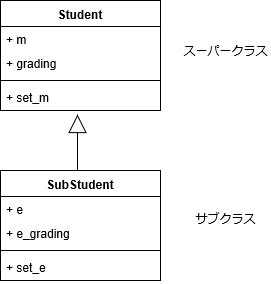
\includegraphics[width=5cm]{images/ClassExtends.png}
\end{center}

サブクラスではスーパークラスの機能を利用することができますので、Studentクラスで定義されているset\_mメソッドやgradingといったデータは
SubStudentクラスで定義していなくても利用できます。
\newpage
{\gt 凡例class-4}
凡例class-3のStudentは(Mathematics)クラスはそのままに(English)の点数のデータを処理し合格"good"か不合格"bad"を判定する
処理set\_eをサブクラスSubStudentに記述します。

{\gt 凡例class1-4.py}
\begin{listing}{1}
class Student: 
    def set_m(self,m):
        self.m = m
        if m >= 50:
            self.grading = "good"
        else:
            self.grading = "bad"
#クラス宣言の括弧の中に利用したい機能のスーパークラスを記載します。
class SubStudent(Student): 
    def set_e(self,e):
        self.e = e
        if e >= 50:
            #合否を実体のデータe_gradingとして設定
            self.e_grading = "good"
        else:
            self.e_grading = "bad"
a = SubStudent()
a.set_m(80)
a.set_e(30)
print("a Mathematics", a.m ,a.grading)
print("a English", a.e ,a.e_grading)
\end{listing}
実行結果
\begin{listing}{1}
a  Mathematics 80 good
a  English 30 bad
\end{listing}







\newpage
\chapter{練習問題解答}


\section{plactice1.py}
\begin{listing}{1}
x = 3
y = 4
print ( (x * y) /2)
\end{listing}


\section{plactice2.py}
\begin{listing}{1}
x = 60
if x >= 50:
    print ( " goukaku " ) 
else:
    print ( " fugoukaku " )
\end{listing}


\section{plactice3.py}
\begin{listing}{1}
x = 1 
y = 2
#それぞれ大小等しいとなる値は何でも構いません
if x > y:
	print("x is large.")
elif x < y:
	print("y is large.")
else:
	print("x and y are equal.")
\end{listing}


\section{plactice4.py}
\begin{listing}{1}
x = 60
if 100 >= x >= 80:
    print ( “A” )
elif x >= 60:
    print ( “B” )
elif x >= 40:
    print ( “C” )
elif x >= 0:
    print ( “D” )
else:
    print ( “error” )
\end{listing}




\section{plactice5.py}
\begin{listing}{1}
x = input ( “math = “ )
m = int ( x ) 
e = input ( “english = “ )
f = int ( e )
z = input ( “social = “ )
s = int ( z )
print ( (m + e + s) / 3 )
\end{listing}


\section{plactice6.py}
\begin{listing}{1}
for x in range(1000):
    print( “wan” )
    print( “nyan” )
\end{listing}



\section{plactice7.py}
\begin{listing}{1}
sum = 0
for x in range(1,1000):
    sum = sum + x
print ( sum ) 

sum = 0
for x in range(1, 11):
    sum = sum + 1 / 2 ** x
print ( sum )
\end{listing}


\section{plactice8.py}
\begin{listing}{1}
y = 0
for n in range(1,6):
    x = input ( “subject” + str(n) + “ = “ )
    y = y + int( x )
print( y / 5 )
\end{listing}


\section{plactice9.py}
\begin{listing}{1}
subjects = ["Mathematics" ,"English","Social","Japanese","Scientific"]
scores = []
for s in subjects:
    x = input( s + " = " )
    y = int ( x )
    if y > 100 or y < 0 :
        y = -1
        print ( "error" )
    scores.append( y )

for n in range(0,5):
    if scores[n] == -1:
        mes = "error"
    elif scores[n] >= 80:
        mes = "excelent"
    elif scores[n] >= 60:
        mes = "good"
    elif scores[n] >= 40:
        mes = "passing"
    else:
        mes = "failing"
    print ( subjects[n] + ":" , scores[n], mes )
\end{listing}


\section{plactice10.py}
\begin{listing}{1}
students_scores = []
#配列の準備
students_scores.append([60, 80]) #Aさんのデータを追加
students_scores.append([70, 90]) #Bさんのデータを追加
students_scores.append([80, 100]) #Cさんのデータを追加
students_scores.append([50, 70]) #Dさんのデータを追加
students_scores.append([60, 60]) #Eさんのデータを追加

m = 0
e = 0

for v in students_scores:
    m = m + v[0]
    e = e + v[1]

print("数学の平均点", m / len(students_scores))
print("英語の平均点", e / len(students_scores))
\end{listing}


\section{plactice11.py}
\begin{listing}{1}
subjects = ["Mathematics" ,"English","Social","Japanese","Scientific"]
scores = []
for n in range(3):
    print(n + 1, "人目の入力")
    scores.append([])
    for s in subjects:
        x = input( s + " = " )
        y = int ( x )
        if y > 100 or y < 0 :
            y = -1
            print ( "error" )
        scores[n].append( y )
s_l = len(subjects) #科目数の取得

for m in range(s_l):
    sum = 0
    m_l = len(scores) #人数の取得
    for n in range(m_l):
        sum = sum + scores[n][m]
    print(subjects[m] , "の平均点", sum / 3)
\end{listing}


\section{plactice12.py}
\begin{listing}{1}
def func1(n):
    a = (n - 65)**2
    return a

def func2():
    t = 0
    for i in range(5):
        x = input()
        y = int(x)
        t = t + func1(y)
    return t

z = func2()
print( z / 5 )
\end{listing}


\section{plactice13.py}
\begin{listing}{1}
#グローバル変数(配列)の準備
subjects = ["Mathematics" ,"English","Social","Japanese","Scientific"]
scores = []
#関数input_dataの記述
def input_data():
    for n in range(3):
        cnt = 0
        scores.append([])
        name = input("Name = ")
        scores[n].append(name)
        for s in subjects:
            x = input( s + " = " )
            y = int ( x )
            if y > 100 or y < 0 :
                y = -1
                print ( "error score" )
            else:
                cnt = cnt + 1
            scores[n].append( y )
        scores[n].append(cnt)
#関数get_averageの記述
def get_average(m):
    sum = 0
    for n in range(1,6):
        if scores[m][n] != -1:
            sum = sum + scores[m][n]
    return sum / scores[m][6]

#プログラムはここから開始
input_data()
for m in range(3):
    ave = get_average(m)
    print(scores[m][0],"の",scores[m][6],"科目の平均点",ave)
\end{listing}


\end{document}